\section{理论基础与带动态误差修正机制的股指波动率预测模型}

本节介绍本文实证分析所使用的主要模型、预测设计与评价指标。本节在统一评价框架中考察点预测与区间预测的不同表现。为此，本文提出一种基于 XGBoost 框架的二段式误差修正模型 XGB-MIDAS-EPU-DEC，该模型通过 MIDAS 方法融合月度经济政策不确定性（EPU）数据，实现对基础模型预测误差的动态修正。本节首先系统梳理各类预测模型的数理基础，随后介绍了所采用的评价指标与方法。最后，本节将对样本划分和评价标准进行阐述。

\subsection{预测目标与基本符号}

设 \(C_t\) 表示第 \(t\) 个交易日的收盘价，日对数收益率 $r_t$ 定义为
\begin{equation}
	r_t=\ln\left(\frac{C_t}{C_{t-1}}\right).
\end{equation}
由于本文使用日度数据，无法直接基于高频日内收益率构造已实现波动率（realized volatility），因此采用日度平方收益率作为波动率代理变量：
\begin{equation}
	RV_t=r_t^2.
\end{equation}
为降低平方收益率分布偏态和极端值影响，并避免对零取对数，本文将一步超前对数波动率 $y_{t+1}$ 定义为主要预测目标：
\begin{equation}
	y_{t+1}=\ln(RV_{t+1}+\varepsilon),
	\qquad \varepsilon=10^{-8}.
\end{equation}
其中，\(\varepsilon\) 为极小正数。除特别说明外，本文所有点预测模型均以 \(y_{t+1}\) 为预测对象。对于需要在原始波动率尺度计算的指标，本文将对数预测值反变换为
\begin{equation}
	\widehat{RV}_{t+1|t}
	=
	\max\left\{
	\exp(\hat{y}_{t+1|t})-\varepsilon,\,
	10^{-12}
	\right\}.
\end{equation}

\paragraph{预测对象与反变换的限制}
平方收益率是条件二阶矩的噪声代理；仅在条件均值为零时，其条件期望等于条件方差。对数MSE训练趋向于条件对数均值，而指数反变换并不等于方差条件均值（Jensen不等式）。GARCH则直接预测条件方差。因而不同模型在MSE与QLIKE下的排序差异，部分可能来自预测目标和反变换差异，不能全部解释为算法优劣。区间覆盖对象是未来平方收益率的对数代理，而不是不可观测条件方差本身。\par

\subsection{基准模型}

金融资产收益率序列通常具有尖峰厚尾、波动聚集和条件异方差等典型特征。相应地，波动率预测模型需要能够刻画波动率的持续性、历史冲击影响以及条件方差动态。本文选取类 HAR 日度波动率模型和 GARCH(1,1) 模型作为传统基准模型，分别对应多尺度波动持续性和条件异方差递推机制。

\subsubsection{类 HAR 模型}

Corsi 提出的 HAR-RV 模型通过日度、周度和月度三个波动率成分近似刻画波动率的长期记忆特征，是波动率预测研究中的经典基准模型 \citep{Corsi2009}。原始 HAR-RV 模型通常基于高频数据构造已实现波动率。考虑到本文使用日度数据，本文借鉴 HAR 的多尺度思想，以平方收益率 \(RV_t=r_t^2\) 作为日度波动率代理。

定义过去 5 日和 22 日平均波动率分别为
\begin{equation}
	\overline{RV}_{t,5}
	=
	\frac{1}{5}\sum_{j=0}^{4}RV_{t-j},
	\qquad
	\overline{RV}_{t,22}
	=
	\frac{1}{22}\sum_{j=0}^{21}RV_{t-j}.
\end{equation}
则本文使用的类 HAR 日度波动率模型设定为
\begin{equation}
	y_{t+1}
	=
	\beta_0
	+
	\beta_d \ln(RV_t+\varepsilon)
	+
	\beta_w \ln(\overline{RV}_{t,5}+\varepsilon)
	+
	\beta_m \ln(\overline{RV}_{t,22}+\varepsilon)
	+
	u_{t+1}.
\end{equation}
其中，日度、周度和月度波动率成分分别刻画短期冲击、中短期波动背景和中期波动状态。该模型结构简单、解释明确，因此适合作为本文的线性波动率预测基准。

\subsubsection{GARCH(1,1) 模型}

Engle 提出的 ARCH 模型首次将条件方差建模为历史冲击平方的函数，Bollerslev 进一步提出 GARCH 模型，使条件方差同时依赖历史冲击和历史条件方差 \citep{Engle1982,Bollerslev1986}。GARCH(1,1) 模型通过递推结构刻画金融收益率中的波动聚集现象，是条件异方差建模中最常用的基准形式之一。

与现存代码一致，本文采用零条件均值及标准化 Student-t 扰动设定，均值和方差方程为：
\begin{equation}
	r_t=\epsilon_t,
	\qquad
	\epsilon_t=\sqrt{h_t}z_t,
\end{equation}
其中 \(h_t\) 为条件方差，\(z_t\) 为均值为 0、方差为 1 的标准化扰动项。GARCH(1,1) 条件方差方程为
\begin{equation}
	h_t
	=
	\omega
	+
	\alpha \epsilon_{t-1}^{2}
	+
	\beta h_{t-1},
	\qquad
	\omega>0,\quad \alpha\geq0,\quad \beta\geq0.
\end{equation}
在标准GARCH假设下，为获得有限的无条件二阶矩，通常要求
\begin{equation}
	\alpha+\beta<1.
\end{equation}
在一步超前预测中，若 \(E(z_t^2)=1\)，则
\begin{equation}
	E(r_{t+1}^{2}\mid \mathcal{F}_t)=h_{t+1}.
\end{equation}
因此，GARCH(1,1) 的一步超前对数波动率预测 $\hat{y}^{GARCH}_{t+1|t}$ 定义为
\begin{equation}
	\hat{y}^{GARCH}_{t+1|t}
	=
	\ln(\hat{h}_{t+1|t}+\varepsilon).
\end{equation}
本文不进一步引入 EGARCH、GJR-GARCH 等扩展模型，原因在于本文目标不是穷尽 GARCH 模型族，而是在统一预测框架下比较传统强基准、机器学习基准和本文提出的两阶段修正模型。

\subsection{基于 MIDAS-EPU 动态误差修正的 XGBoost 波动率预测模型}

本文提出基于 MIDAS-EPU 动态误差修正的 XGBoost 波动率预测模型，即 XGBoost Volatility Forecasting Model with MIDAS-EPU Dynamic Error Correction，简称 XGB-MIDAS-EPU-DEC。该模型采用两阶段结构：第一阶段首先使用日度市场变量构建 XGB-Market 机器学习基准预测，随后在第二阶段利用历史样本外预测残差和 MIDAS 加权的月度经济政策不确定性信息构造动态误差修正项。最终预测由第一阶段基准预测与第二阶段误差修正项相加得到。

\subsubsection{XGB-Market 基准模型}

XGBoost 是一种基于梯度提升树的集成学习方法，能够通过逐步叠加回归树逼近复杂非线性函数，并在目标函数中加入正则化项以控制模型复杂度 \citep{ChenGuestrin2016}。与线性模型相比，XGBoost 能够更灵活地刻画变量之间的非线性关系和交互效应，因此适合用于包含多类市场特征的波动率预测任务。

设 \(X_t^M\) 表示第 \(t\) 个交易日可观测的日度市场特征向量，包括历史波动率、收益率、价格振幅和成交量等变量。第一阶段 XGB-Market 模型可表示为
\begin{equation}
	\hat{y}^{XGB}_{t+1|t}
	=
	f_{XGB}(X_t^M),
\end{equation}
其中 \(f_{XGB}(\cdot)\) 表示由训练样本估计得到的非线性映射函数。本文将 XGB-Market 作为机器学习基准模型，用于检验仅依赖日度市场变量的非线性模型是否能够提供样本外预测增益。

\subsubsection{MIDAS-EPU 变量构造}

本文使用的经济政策不确定性指数为月度频率，而股指市场变量为日度频率，因此二者构成混频数据结构。若直接将月度 EPU 简单填充至日度样本，难以刻画低频变量的滞后影响；若直接纳入多个滞后月份变量，则可能造成参数过多和样本效率下降。MIDAS 方法通过参数化权重函数将低频变量的多期滞后压缩为少量参数，适用于处理不同频率变量之间的预测关系 \citep{GhyselsSinkoValkanov2007,EngleGhyselsSohn2013}。

设交易日 \(t\) 所属自然月份为 \(m(t)\)。现存代码不使用当月 EPU，而按月份标签使用 \(m(t)-1\) 及更早月份的信息。月份滞后并不能证明实际发布日期之前可得；未保存逐日发布日与历史修订版本，因此这里只能称为回顾性伪样本外实验。给定滞后长度 \(K\)，MIDAS-EPU 指标 $\widetilde{EPU}_{t}^{(K,\boldsymbol{\theta})}$ 定义为
\begin{equation}
	\widetilde{EPU}_{t}^{(K,\boldsymbol{\theta})}
	=
	\sum_{k=1}^{K}
	w(k;\boldsymbol{\theta})
	\ln(EPU_{m(t)-k}),
\end{equation}
其中 \(w(k;\boldsymbol{\theta})\) 为权重函数，并满足
\begin{equation}
	w(k;\boldsymbol{\theta})\geq0,
	\qquad
	\sum_{k=1}^{K}w(k;\boldsymbol{\theta})=1.
\end{equation}
本文主要考虑 Beta 权重和指数 Almon 权重两类常见 MIDAS 权重函数。Beta 权重定义为
\begin{equation}
	w^{B}(k;\theta_1,\theta_2)
	=
	\frac{a_k}{\sum_{j=1}^{K}a_j},
    \quad a_k=\max\{x_k^{\theta_1-1}(1-x_k)^{\theta_2-1},10^{-12}\},
	\qquad
	x_k=\frac{K-k+1}{K+1}.
\end{equation}
为与保存的权重及参数一致，令 $z_k=(K-k+1)/K$，指数 Almon 权重定义为
\begin{equation}
	w^{EA}(k;\theta_1,\theta_2)
	=
	\frac{
		\exp(\theta_1 z_k+\theta_2 z_k^2)
	}{
		\sum_{j=1}^{K}\exp(\theta_1 z_j+\theta_2 z_j^2)
	}.
\end{equation}

\subsubsection{XGB-MIDAS-EPU-DEC 动态误差修正模型}

第一阶段 XGB-Market 模型生成基准预测值后，本文进一步构造其样本外预测残差。设第一阶段模型在时点 \(t-1\) 对 \(y_t\) 的预测为 \(\hat{y}^{XGB}_{t|t-1}\)，则样本外残差 $e_t$ 定义为
\begin{equation}
	e_t
	=
	y_t-\hat{y}^{XGB}_{t|t-1}.
\end{equation}
其中 \(e_t\) 必须是真实样本外残差，而不是样本内拟合残差。若使用样本内残差训练第二阶段模型，可能会将第一阶段模型的过拟合误差误认为可利用的动态结构，从而高估模型的预测能力。

第二阶段误差修正模型设定 $e_{t+1}$ 为
\begin{equation}
	e_{t+1}
	=
	\alpha_0
	+
	\rho e_t
	+
	\gamma
	\widetilde{EPU}_{t}^{(K,\boldsymbol{\theta})}
	+
	u_{t+1}.
	\label{eq:error_correction}  
\end{equation}
式 \eqref{eq:error_correction} 本质上是一个 ARX(1) 回归模型，用于预测 $e_{t+1}$。其中，\(e_t\) 反映预测误差的短期持续性，\(\widetilde{EPU}_{t}^{(K,\boldsymbol{\theta})}\) 表征低频政策不确定性与预测偏差的滞后关联。最终预测值 $\hat{y}^{final}_{t+1|t}$ 为
\begin{equation}  
	\hat{y}^{final}_{t+1|t}
	=
	\hat{y}^{XGB}_{t+1|t}
	+
	\hat{e}_{t+1|t}.
\end{equation}

该框架的主要特点是将“日度市场变量的非线性预测能力”和“月度政策不确定性的误差修正作用”分层建模。第一阶段负责提取市场变量中的非线性信息，第二阶段检验历史残差与EPU组合的预测表现，不能仅凭该组合识别EPU单独贡献。需要注意的是，第二阶段中的残差 \(e_t\) 属于生成回归量，相关系数不宜解释为严格因果效应 \citep{Pagan1984}。因此，本文关注的是该修正机制能否改善样本外预测表现，而非识别 EPU 对股指波动率的结构性因果效应。

\paragraph{第二阶段的修订估计与规格选择}
给定窗口$K$、权重族及形状参数$\theta$，线性系数通过OLS估计。将剖面目标写为
\[
 F(\theta)=n^{-1}\min_{a,\rho,\gamma}\|e-a\mathbf1-\rho e_{-1}-\gamma Lw(\theta)\|^2.
\]
其中$L$为训练段月度对数EPU滞后矩阵。通过SVD将$e$及$L$投影到截距和滞后残差的正交补，消去线性控制项；这种变量投影思路用于可分离非线性最小二乘\citep{GolubPereyra1973}。设最优线性回归残差为$r$，在秩不变且权重可微处，剖面梯度为
\[
 \nabla_\theta F=-\frac{2\hat\gamma}{n}\left(L\frac{\partial w}{\partial\theta}\right)^\top r.
\]
Beta仍保留归一化前$10^{-12}$下截；低于阈值的原始权重导数设为零，阈值处为分段可微。本文没有改变权重族或参数范围来追求测试指标。

旧版使用单起点L-BFGS-B、前向差分及默认相对目标停止阈值；部分成功标志没有对应足够小的梯度，且可能停在不同局部解。修订版最小化平均平方残差并传入解析梯度。Beta两参数范围均为$[0.05,20]$，采用$\{0.05,0.5,1.5,5,20\}\times\{0.05,0.5,2,5,20\}$的25个起点；指数Almon范围均为$[-5,5]$，采用$\{-5,-2.5,0,2.5,5\}^2$及旧起点$(-0.2,-0.02)$，共26个起点。L-BFGS-B的$ftol=10^{-14}$、$gtol=10^{-9}$、最大迭代2000、最大函数调用10000、最大线搜索50。投影梯度超过$10^{-6}$时从该候选点用SLSQP重试。每次选择训练目标最低的候选；若该解仍不满足$10^{-6}$验收阈值则报错，不据测试表现替换解。停止规则的区别见SciPy官方说明\footnote{\url{https://docs.scipy.org/doc/scipy/reference/optimize.minimize-lbfgsb.html}}。

第一阶段顺序生成500条验证样本的样本外预测。构造一阶残差滞后后，499条有效残差按时间分为299条估计与200条评分。对$K\in\{6,12,24\}$及两种权重族共六组规格，按后200条残差预测MSE选取；评分段使用已实现的前期残差，参数不重估。测试期固定窗口和权重族，每60条保留观测重新估计形状参数及线性系数，训练只包含此前已经实现的样本外残差。求解规则在本轮新测试结果产生前固定，但历史结果已被查看，故本轮属于回顾性方法修订，不是预注册验证。

\paragraph{残差单独修正的消融对照}
新增XGB-AR：$\hat y^{AR}_{t+1|t}=\hat y^{XGB}_{t+1|t}+\hat a+\hat\rho e_t$。它不含EPU，使用与DEC相同的可用历史残差、扩展窗口及60条重估间隔，以OLS估计，没有新增调参。DEC与XGB-AR的比较用于评价该设定下加入EPU的增量表现；它仍不能识别外生政策冲击、排除数据版本问题或建立因果关系。

\subsection{研究假设}

基于上述理论机制与模型设定，本文并不预设复杂模型必然优于传统模型，而是在统一的样本外预测框架下检验不同信息来源和模型结构是否具有增量预测价值。具体而言，本文遵循以下研究假设。

\textbf{假设 H1：股指波动率具有持续性与多尺度依赖结构。}

金融资产收益率通常存在波动聚集和条件异方差特征，意味着高波动状态往往会在短期内延续，低波动状态也具有一定持续性。同时，不同期限投资者的信息处理周期和交易行为存在差异，使得未来波动率可能同时受到日度、周度和月度历史波动状态的影响。因此，本文预期基于历史波动率构造的 HAR 类变量能够为下一期波动率预测提供有效信息。

\textbf{假设 H2：日度市场变量中存在可由非线性模型捕捉的预测信息。}

传统线性模型虽然具有较强解释性，但其对变量间非线性关系和交互效应的刻画能力有限。股指波动率可能同时受到历史波动、收益率冲击、价格振幅和成交量变化等多类市场变量影响，且这些变量之间的关系未必满足简单线性形式。因此，本文预期 XGB-Market 模型能够从日度市场变量中提取一定非线性预测信息，但其样本外表现仍需与 HAR 和 GARCH 等传统强基准进行比较。

\textbf{假设 H3：经济政策不确定性包含股指波动率预测的增量信息。}

经济政策不确定性可能通过影响投资者预期、风险补偿要求、市场流动性和交易行为等渠道改变股票市场风险状态。由于政策信息从形成、传播到被市场吸收通常存在一定时滞，EPU 对股指波动率的影响未必表现为即时冲击，而可能具有滞后性和持续性。因此，本文预期经过 MIDAS 权重重构的 EPU 信息能够解释第一阶段市场模型未能捕捉的部分系统性预测误差。

\textbf{假设 H4：动态误差修正能够改善单一机器学习模型的样本外预测表现。}

如果 XGB-Market 的样本外预测残差并非纯随机噪声，而是仍包含残差持续性或低频政策不确定性信息，则在第一阶段预测基础上引入动态误差修正项应当能够改善最终预测结果。基于此，本文预期 XGB-MIDAS-EPU-DEC 模型相对于单一 XGB-Market 模型具有一定增量预测价值，并可能在点预测精度与区间预测表现之间取得相对平衡。

本轮用XGB-AR进行EPU消融比较，但H3的判断仍须区分损失函数和市场，不能把局部指标改善解释为全面预测优势。需要说明的是，上述假设均属于预测意义上的经验假设，而非严格因果识别命题。本文关注的是不同变量和模型结构是否能够在样本外预测中提供有效增量信息，而不将 EPU 系数或误差修正项解释为政策不确定性对股指波动率的结构性因果效应。

\subsection{XGB-Market 模型变量构造}

被解释变量的设定与前文相同，即核心预测对象为下一交易日对数波动率。

解释变量主要由日度市场变量构造，包括三类。第一类为多尺度历史波动率变量，用于刻画波动率持续性：
\begin{equation}
	\ln RV_t=\ln(RV_t+\varepsilon),
\end{equation}
\begin{equation}
	\ln \overline{RV}_{t,5}
	=
	\ln\left(\frac{1}{5}\sum_{i=0}^{4}RV_{t-i}+\varepsilon\right),
\end{equation}
\begin{equation}
	\ln \overline{RV}_{t,22}
	=
	\ln\left(\frac{1}{22}\sum_{i=0}^{21}RV_{t-i}+\varepsilon\right).
\end{equation}
第二类为收益率方向变量：
\begin{equation}
	r_t^{+}=\max(r_t,0),\qquad
	r_t^{-}=\min(r_t,0).
\end{equation}
第三类为价格振幅和成交量变量。设 \(H_t\)、\(L_t\)、\(V_t\) 分别表示第 \(t\) 个交易日最高价、最低价和成交量，则日内振幅 $R_t$ 定义为
\begin{equation}
	R_t=\ln\left(\frac{H_t}{L_t}\right),
\end{equation}
短期振幅均值 $\overline{R}_{t,5}$ 定义为
\begin{equation}
	\overline{R}_{t,5}
	=
	\frac{1}{5}\sum_{i=0}^{4}R_{t-i}.
\end{equation}
成交量变量包括对数成交量水平和对数成交量变化率：
\begin{equation}
	\ln V_t,\qquad
	\Delta \ln V_t=\ln V_t-\ln V_{t-1}.
\end{equation}

表 \ref{tab:variables_main} 汇总了本文主要变量定义。

\begin{table}[!htbp]
	\centering
	\makebox[\textwidth][c]{
		\begin{threeparttable}
			\captionsetup{font=small,skip=3pt}
			\caption{主要市场变量定义}
			\label{tab:variables_main}
			
			\begingroup
			\footnotesize
			\setlength{\tabcolsep}{4pt}
			\renewcommand{\arraystretch}{1.13}
			
			\begin{tabularx}{0.90\textwidth}{
					>{\raggedright\arraybackslash}p{2.55cm}
					>{\centering\arraybackslash}p{2.35cm}
					>{\centering\arraybackslash}X
				}
				\toprule
				变量名称 & 符号 & 数学定义 \\
				\midrule
				日对数收益率 & \(r_t\) & \(\ln(C_t/C_{t-1})\) \\
				波动率代理变量 & \(RV_t\) & \(r_t^2\) \\
				一步超前预测目标 & \(y_{t+1}\) & \(\ln(RV_{t+1}+\varepsilon)\) \\
				即时历史波动率 & \(\ln RV_t\) & \(\ln(RV_t+\varepsilon)\) \\
				周度历史波动率 & \(\ln \overline{RV}_{t,5}\) & \(\ln\{5^{-1}\sum_{i=0}^{4}RV_{t-i}+\varepsilon\}\) \\
				月度历史波动率 & \(\ln \overline{RV}_{t,22}\) & \(\ln\{22^{-1}\sum_{i=0}^{21}RV_{t-i}+\varepsilon\}\) \\
				正收益项 & \(r_t^+\) & \(\max(r_t,0)\) \\
				负收益项 & \(r_t^-\) & \(\min(r_t,0)\) \\
				日内振幅 & \(R_t\) & \(\ln(H_t/L_t)\) \\
				短期振幅均值 & \(\overline{R}_{t,5}\) & \(5^{-1}\sum_{i=0}^{4}R_{t-i}\) \\
				成交量水平 & \(\ln V_t\) & \(\ln(V_t)\) \\
				成交量变化率 & \(\Delta\ln V_t\) & \(\ln(V_t)-\ln(V_{t-1})\) \\
				\bottomrule
			\end{tabularx}
			\endgroup
			
			\begin{tablenotes}[flushleft]
				\scriptsize
				\item 注：\(C_t\)、\(H_t\)、\(L_t\) 和 \(V_t\) 分别表示第 \(t\) 个交易日的收盘价、最高价、最低价和成交量；\(\varepsilon=10^{-8}\)，用于避免对零取对数。除一步超前预测目标 \(y_{t+1}\) 外，表中解释变量均为 \(t\) 时点及以前可观测的市场变量，用于第一阶段 XGB-Market 预测模型。EPU 信息不作为本表中的市场解释变量，而是在第二阶段通过 MIDAS-EPU 因子进入动态误差修正模型。
			\end{tablenotes}
		\end{threeparttable}
	}
\end{table}


由于部分解释变量依赖过去 5 个或 22 个交易日的信息，滚动计算会导致样本前段产生不可定义观测；同时，主预测目标 \(y_{t+1}\) 需要使用下一交易日收益率，因此样本末端也会自然损失少量观测。本文在建模前统一删除由变量构造导致的缺失观测。此类处理并非对原始数据进行插补或平滑，而是由预测变量定义和超前目标构造自然决定。

本文的核心任务是预测股指下一交易日对数波动率，并在统一的伪样本外框架下比较传统波动率模型、机器学习基准模型以及本文提出的 XGB-MIDAS-EPU-DEC 模型。为避免不同章节之间重复，本节不再展开数据来源和具体变量清洗过程，而是重点说明模型设定、预测目标、样本外预测原则以及点预测和区间预测的评价方法。

\subsection{数据来源与样本处理}

本文使用CSI300日度行情，字段包括日期、开高低收与成交量，范围为2010年1月至2026年3月。现存输入有3942条价格，按相邻收盘价比值计算并删除首个不可定义值后，得到3941条收益率。公开版的描述统计、检验及相应图件均据此重新生成。历史3942条统计可由在2018年6月15日与6月19日收益率之间额外插入一个零值精确重构，包括10项描述统计及JB、Ljung--Box、ARCH检验，共24个数值；插入操作仅用于追查，未作为真实数据使用。额外记录的原始日期及形成过程没有保存，不能认定为某个交易日或首行填充值。

三个指数的日期、全部市场特征、24个月EPU滞后及训练/验证/测试划分均可由现存输入重建，与保存的建模矩阵在数值容差内一致。CSI300建模矩阵为3919行，未包含上述额外零值；描述统计差异不能据此归结为最终预测输入错配。

经济政策不确定性变量采用 Davis、Liu 和 Sheng 基于中国大陆报纸构造的中国经济政策不确定性指数（China Economic Policy Uncertainty Index, China EPU）月度数据 \citep{DavisLiuSheng2019}。由于市场数据为日度频率，而 EPU 数据为月度频率，代码以月度滞后对齐EPU；没有原始发布日与修订版本，不能独立证明实时可得性。行情预测原点为交易日收盘后。

\subsection{数据统计学特征检验}

为确认主样本是否具有典型金融时间序列特征，本文对 CSI 300 日对数收益率进行描述性统计、正态性检验、自相关检验和条件异方差检验。表 \ref{tab:desc_return_short} 汇报了日对数收益率的主要描述性统计结果。

\begin{table}[!htbp]
	\centering
	\caption{CSI 300 日对数收益率描述性统计（3941条收益率，已复算）}
	\label{tab:desc_return_short}
	\begingroup
	\footnotesize
	\setlength{\tabcolsep}{5pt}
	\renewcommand{\arraystretch}{1.08}
	\begin{tabular}{lcccccc}
		\toprule
		样本量 & 均值 & 标准差 & 最小值 & 最大值 & 偏度 & 超额峰度 \\
		\midrule
		3941 & \(5.8396\times10^{-5}\) & 0.013639 & -0.091544 & 0.081420 & -0.576130 & 5.460548 \\
		\bottomrule
	\end{tabular}
	\endgroup
\end{table}

结果显示，CSI 300 日对数收益率均值接近零，标准差为 0.013639；收益率分布存在左偏，样本超额峰度大于零，说明样本具有尖峰厚尾特征。如图 \ref{fig:return_ts_qq}，提供了尖峰厚尾特征的图像证据。为进一步检验收益率序列的分布和动态依赖性质，本文报告 Jarque--Bera 检验、Ljung--Box 检验和 ARCH-LM 检验结果，如表 \ref{tab:diagnostic_tests_short} 所示。

\begin{table}[!htbp]
	\centering
	\caption{CSI 300 日对数收益率统计特征检验（3941条收益率，已复算）}
	\label{tab:diagnostic_tests_short}
	\footnotesize
	\setlength{\tabcolsep}{6pt} 
	\renewcommand{\arraystretch}{1.08}
	\begin{tabular}{l c c r} 
		\toprule
		检验 & 对象/滞后阶数 & 统计量 & \(p\)-value \\
		\midrule
		Jarque--Bera & \(r_t\) & 5099.01 & $<0.0001$ \\
		Ljung--Box & \(r_t\), 10阶 & 32.75 & 0.0003 \\
		Ljung--Box & \(r_t\), 20阶 & 64.45 & \(1.43\times10^{-6}\) \\
		Ljung--Box & \(r_t^2\), 10阶 & 1051.71 & \(1.35\times10^{-219}\) \\
		Ljung--Box & \(r_t^2\), 20阶 & 1526.13 & \(9.87\times10^{-312}\) \\
		ARCH-LM & 10阶 & 452.36 & \(6.56\times10^{-91}\) \\
		ARCH-F & 10阶 & 50.98 & \(9.52\times10^{-97}\) \\
		\bottomrule
	\end{tabular}
\end{table}

\begin{figure}[H]
	\centering 
	\subfigure[CSI 300 日对数收益率时序图]{ 
		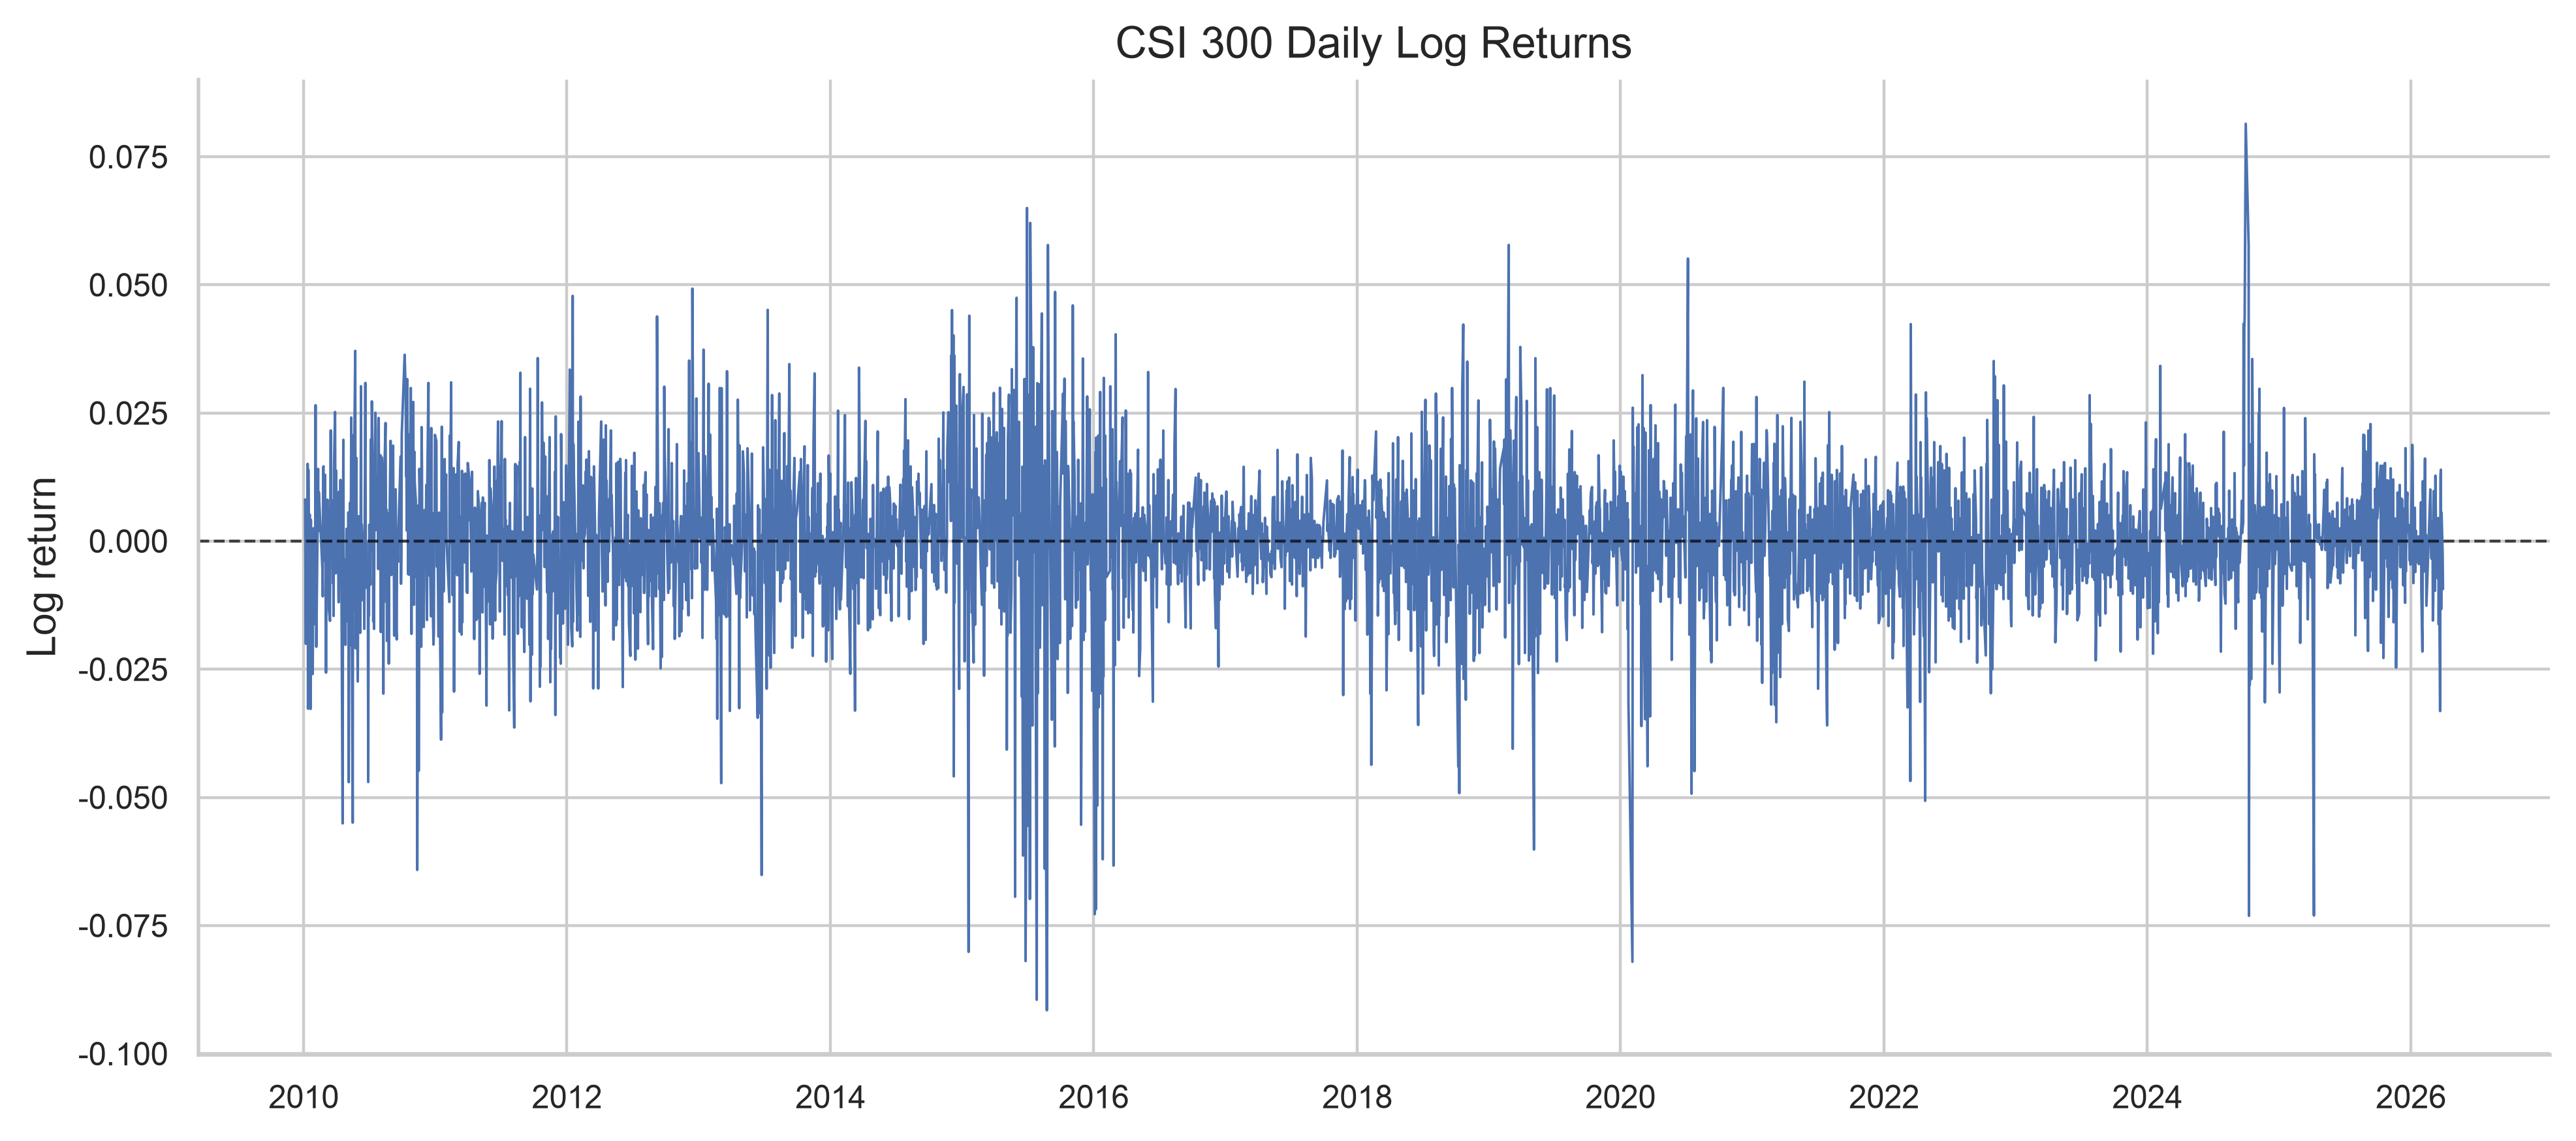
\includegraphics[width=0.47\textwidth]{../../results/descriptive-corrected/figure_1_log_return_series.png} } 
	\hfill 
	\subfigure[CSI 300 日对数收益率 QQ 图]{ 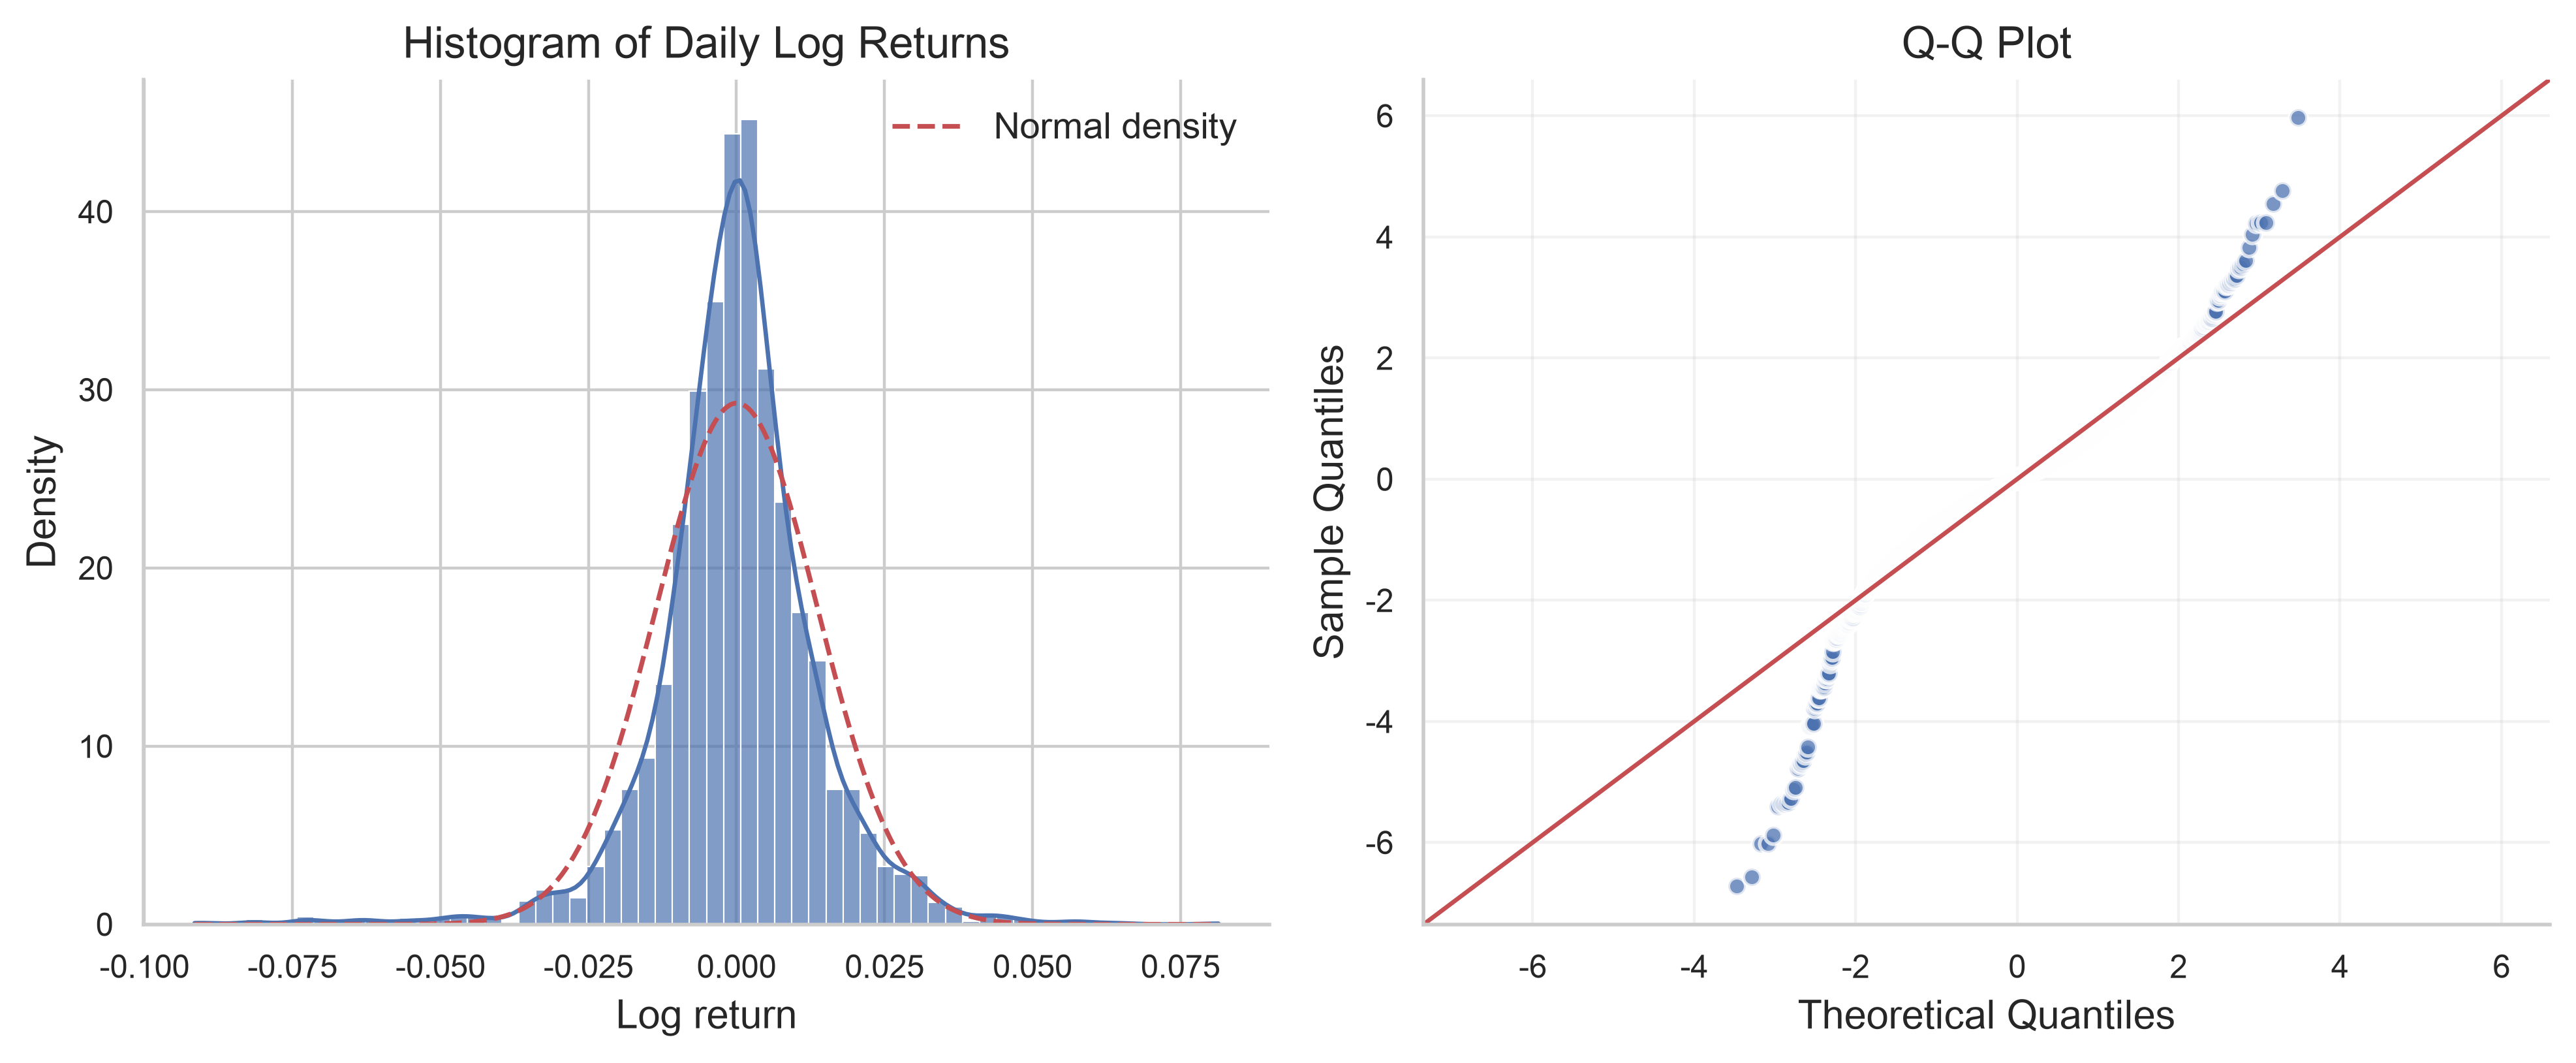
\includegraphics[width=0.47\textwidth]{../../results/descriptive-corrected/figure_2_histogram_qq.png} } 
	\caption{CSI 300 日对数收益率序列图形特征} 
	\label{fig:return_ts_qq} 
\end{figure}

Jarque--Bera 检验拒绝收益率正态分布假设；平方收益率的 Ljung--Box 检验在所报告滞后下拒绝无自相关原假设，提示波动率代理序列存在序列依赖；ARCH-LM 检验显著拒绝同方差假设，表明收益率序列具有条件异方差特征。上述结果为后续使用 HAR 类变量、GARCH 模型和非线性预测模型提供了经验依据。

\subsection{伪样本外预测设计}

在预测过程中，本文采用一步超前预测框架。设 \(\mathcal{F}_t\) 表示时点 \(t\) 已经可获得的信息集，则所有模型在预测 \(y_{t+1}\) 时只能使用 \(\mathcal{F}_t\) 中的信息：
\begin{equation}
	\hat{y}_{t+1|t}
	=
	g(\mathcal{F}_t).
\end{equation}
随着时间推进，训练窗口逐步向前扩展。对于 HAR 和 GARCH(1,1) 模型，本文在扩展窗口内递推估计模型参数并生成一步超前预测；对于 XGB-Market 模型，本文使用固定300轮、深度4等附录配置，在扩展窗口中每20条保留观测重训，不采用固定长度滚动窗口或早停；对于 XGB-MIDAS-EPU-DEC 模型，第二阶段误差修正层仅使用已经实现的历史样本外残差。

伪样本外预测设计的关键在于信息集闭合。尤其对于本文的两阶段模型，第二阶段误差修正不能使用尚未实现的残差。只有当 \(y_t\) 实现之后，残差
\begin{equation}
	e_t=y_t-\hat{y}_{t|t-1}
\end{equation}
才可以作为时点 \(t\) 之后的可用信息进入误差修正模型。该处理是避免前视偏差和样本内过拟合的重要条件。

\paragraph{代码行号、缺失行与交易日历限制}
代码中日期为 $t$ 的行保存的是超前目标 $y_{t+1}$；第一阶段重训使用该行之前的行，其最后一个目标在收盘时已经实现。第二阶段同样在预测原点前截断训练行。市场特征仅作本文所列对数、滚动均值和缺失处理，匹配存档的主流程没有缩尾、标准化或第一阶段内部早停。这里的20与60为过滤后行数，存在缺口时不应直接称为20或60个连续交易日。

此外，历史代码先在原价格行上计算收益率与超前目标，再删除缺失特征行；残差滞后则对保留行作一次位移。无缺口时它等于式\eqref{eq:error_correction}中的 $e_t$；有缺口时应理解为最近保留预测所对应、已经实现的残差，并不一定是紧邻交易日残差。上证50历史测试段的2018年6月25日存在一处这种情况；本轮先删除确认的休市行后该处缺口消失。其他零成交量及缺失特征仍需完整日历审计。

上证50源表还把2018年6月18日列为与前一行同收盘价、零成交量的记录，而上交所公告确认该日休市\footnote{上海证券交易所《关于上海证券交易所2018年全年休市安排的通知》，2017-12-22，公告〔2017〕26号，端午节安排。}。尽管该行的缺失成交量特征后来被删除，6月15日行的超前目标仍指向它，产生 $\ln(10^{-8})$ 的人工零收益目标，并影响相邻滚动特征。因此，“下一交易日”是研究设计目标，并非上证50历史数据所有行都满足的已验证事实。历史结果保留在归档目录；本文正文的修订上证50实验先排除该休市行，重建收益率、目标及特征，再生成全部基准和修正模型预测。修订样本为1500/500/1919，不能只删一条测试损失代替重估。附录另保留上一轮日历清洗对照。其他零成交量记录不凭此一项特征认定为休市。

\subsection{波动率点预测评价方法}

\subsubsection{MSE 与 MAE}

本文首先使用均方误差（Mean Squared Error, MSE）和平均绝对误差（Mean Absolute Error, MAE）评价模型在对数波动率代理尺度上的预测精度。设测试集共有 \(N\) 个预测观测，真实值为 \(y_{t+1}\)，预测值为 \(\hat{y}_{t+1|t}\)，则
\begin{equation}
	MSE
	=
	\frac{1}{N}
	\sum_{t=1}^{N}
	\left(
	y_{t+1}-\hat{y}_{t+1|t}
	\right)^2,
\end{equation}
\begin{equation}
	MAE
	=
	\frac{1}{N}
	\sum_{t=1}^{N}
	\left|
	y_{t+1}-\hat{y}_{t+1|t}
	\right|.
\end{equation}
MSE 对极端误差更敏感，MAE 则更直接反映平均绝对偏离。二者结合可以从不同角度评价模型在对数波动率代理尺度上的预测表现。

\subsubsection{QLIKE 损失函数}

由于真实条件方差无法直接观测，波动率预测通常需要借助代理变量进行评价。Patton 指出，在波动率代理变量存在测量误差时，损失函数的选择可能影响模型排序，QLIKE 损失函数在波动率预测评价中具有在代理条件无偏等前提下的排序稳健性 \citep{Patton2011}。因此，本文将 QLIKE 作为重要补充指标。

设真实波动率代理为 \(RV_{t+1}\)，模型预测方差为 \(\widehat{RV}_{t+1|t}\)，则 QLIKE 定义为
\begin{equation}
	QLIKE
	=
	\frac{1}{N}
	\sum_{t=1}^{N}
	\left[
	\frac{RV_{t+1}}{\widehat{RV}_{t+1|t}}
	-
	\ln
	\left(
	\frac{RV_{t+1}}{\widehat{RV}_{t+1|t}}
	\right)
	-
	1
	\right].
\end{equation}
QLIKE 值越低，表示模型在原始方差尺度上的预测表现越好。实现时，观测代理与预测值在对数反变换后均下截至 $10^{-12}$，再计算比值及其对数；这避免零值导致未定义损失，但属于数值截断，不保证截断后的代理仍满足条件无偏假设。

\subsubsection{损失差与探索性统计诊断}
定义$d_t=L_{A,t}-L_{DEC,t}$，正均值表示DEC的平均损失较低。对每市场、每个损失以及XGB-Market和XGB-AR两个比较对象，报告均值差、Newey--West型HAC标准误及正态参考双侧$p$值\citep{DieboldMariano1995,NeweyWest1987}。Bartlett核带宽为$\lfloor4(N/100)^{2/9}\rfloor$，本次均为7；使用生存函数计算尾概率，避免将数值下溢写成真正的零。三市场、三损失、两比较共18项，统一按Holm方法调整\citep{Holm1979}。

这里涉及扩展估计窗口、生成残差、近似嵌套模型及验证集规格选择。HAC和Holm不能自动消除选择偏差或保证标准预测检验的极限分布适用，因此以上数值仅为损失差的探索性诊断，不作为因果识别或确认性显著性证明。没有在本轮重复报告旧版Clark--West型显著性结论；其普通样本标准误及单侧$t$分布不充分处理这些条件，旧统计量仅在历史档案中保留\citep{ClarkWest2007}。

\subsection{波动率区间预测方法与评价指标}

\subsubsection{滚动共形预测区间}

点预测只能给出未来波动率的中心预测值，无法直接刻画预测不确定性。因此，本文在点预测结果基础上进一步构造滚动共形预测区间。共形预测为模型无关的区间构造提供了通用框架 \citep{Vovk2005,ShaferVovk2008,Lei2018}。不过，标准共形预测通常依赖可交换性假设，而金融时间序列存在自相关、波动聚集和分布漂移。为适应时间序列环境，本文采用滚动校准方式，仅使用近期已经实现的样本外残差构造区间，该思想与时间序列共形预测文献相一致 \citep{XuXie2021}。

设某模型的一步超前预测误差 $e_i$ 为
\begin{equation}
	e_i=y_i-\hat{y}_{i|i-1},
\end{equation}
定义非符合度分数为绝对预测误差：
\begin{equation}
	s_i=|e_i|.
\end{equation}
在预测 \(y_{t+1}\) 时，本文使用时点 \(t\) 之前已经实现的最近 \(m\) 个非符合度分数作为滚动校准集，并计算经验分位数
\begin{equation}
	q_{1-\alpha,t}
	=
	s_{(\lceil(n_t+1)(1-\alpha)\rceil)},
\end{equation}
其中 \(n_t\) 为当前校准窗口内可用分数个数，\(s_{(k)}\) 表示按从小到大排序后的第 \(k\) 个非符合度分数。若阶数超过校准样本数，现存代码截断为最大观测分数；这不构成一般的有限样本覆盖保证。本实验至少60条校准分数、显著性水平0.05或0.10，不触发该截断边界。

在对数波动率代理尺度上，一步超前预测区间的下界与上界分别为
\begin{equation}
	L^{(y)}_{t+1|t}
	=
	\hat{y}_{t+1|t}
	-
	q_{1-\alpha,t},
	\qquad
	U^{(y)}_{t+1|t}
	=
	\hat{y}_{t+1|t}
	+
	q_{1-\alpha,t}.
\end{equation}
若需转换至原始波动率尺度，则有
\begin{equation}
	L^{(RV)}_{t+1|t}
	=
	\max\left\{
	0,\,
	\exp(L^{(y)}_{t+1|t})-\varepsilon
	\right\},
	\qquad
	U^{(RV)}_{t+1|t}
	=
	\max\{0,\exp(U^{(y)}_{t+1|t})-\varepsilon\}.
\end{equation}

需要说明的是，本文不声称滚动共形区间在金融时间序列中严格满足独立同分布条件下的有限样本覆盖保证，而是将其作为一种满足时间顺序约束、具有清晰经验校准逻辑的区间预测方法。

\subsubsection{经验覆盖率}

经验覆盖率用于衡量预测区间实际覆盖真实值的比例。对于名义覆盖率 \(1-\alpha\)，定义
\begin{equation}
	CP_{1-\alpha}
	=
	\frac{1}{N}
	\sum_{t=1}^{N}
	\mathbf{1}
	\left\{
	L^{(y)}_{t+1|t}
	\leq
	y_{t+1}
	\leq
	U^{(y)}_{t+1|t}
	\right\}.
\end{equation}
若 \(CP_{1-\alpha}\) 接近名义覆盖率，则说明预测区间具有较好的经验校准性。

\subsubsection{平均区间宽度}

平均区间宽度 $AW_{1-\alpha}$ 用于衡量预测区间的紧致程度，定义为
\begin{equation}
	AW_{1-\alpha}
	=
	\frac{1}{N}
	\sum_{t=1}^{N}
	\left(
	U^{(y)}_{t+1|t}
	-
	L^{(y)}_{t+1|t}
	\right).
\end{equation}
仅追求高覆盖率可能导致区间过宽，因此覆盖率必须与区间宽度共同考察。

\subsubsection{区间得分}

本文同时采用区间得分作为综合区间评价指标 \citep{GneitingRaftery2007}。对于显著性水平 \(\alpha\)，单期区间得分 $IS_{\alpha,t+1}$ 定义为
\begin{equation}
	\begin{aligned}
		IS_{\alpha,t+1}
		=
		&
		\left(
		U^{(y)}_{t+1|t}
		-
		L^{(y)}_{t+1|t}
		\right)
		\\
		&
		+
		\frac{2}{\alpha}
		\left(
		L^{(y)}_{t+1|t}
		-
		y_{t+1}
		\right)
		\mathbf{1}
		\left\{
		y_{t+1}<L^{(y)}_{t+1|t}
		\right\}
		\\
		&
		+
		\frac{2}{\alpha}
		\left(
		y_{t+1}
		-
		U^{(y)}_{t+1|t}
		\right)
		\mathbf{1}
		\left\{
		y_{t+1}>U^{(y)}_{t+1|t}
		\right\}.
	\end{aligned}
\end{equation}
样本平均区间得分 $\overline{IS}_{\alpha}$ 为
\begin{equation}
	\overline{IS}_{\alpha}
	=
	\frac{1}{N}
	\sum_{t=1}^{N}
	IS_{\alpha,t+1}.
\end{equation}
区间得分同时惩罚区间过宽和覆盖失败，数值越小表示区间预测质量越高。

\subsection{本章小结}

本节给出了本文实证分析所需的理论基础、模型设定与评价方法。首先，类 HAR 模型和 GARCH(1,1) 模型分别从多尺度波动持续性和条件异方差递推角度构成传统基准。其次，XGB-Market 模型用于提取日度市场变量中的非线性预测信息。再次，本文提出 XGB-MIDAS-EPU-DEC 模型，将 MIDAS 加权的月度 EPU 信息置于第二阶段动态误差修正层中，用于检验含EPU和历史残差的组合修正表现；并加入XGB-AR对照评价EPU在该设定下的增量表现。

在研究设计上，本文选用 CSI 300 数据作为主实验数据来源，采用时间顺序下的伪样本外预测框架，按代码时间索引约束训练、调参、残差构造和区间校准；EPU真实发布时点与修订信息未核实。在评价方法上，本文同时使用 MSE、MAE 和 QLIKE 评价点预测表现，并报告HAC损失差和Holm调整的探索性诊断；对于区间预测，本文采用滚动共形预测方法，并使用经验覆盖率、平均区间宽度和区间得分进行评价。上述方法共同构成后续实证分析的统一基础。